% This is "sig-alternate.tex" V2.1 April 2013
% This file should be compiled with V2.5 of "sig-alternate.cls" May 2012
%
% This example file demonstrates the use of the 'sig-alternate.cls'
% V2.5 LaTeX2e document class file. It is for those submitting
% articles to ACM Conference Proceedings WHO DO NOT WISH TO
% STRICTLY ADHERE TO THE SIGS (PUBS-BOARD-ENDORSED) STYLE.
% The 'sig-alternate.cls' file will produce a similar-looking,
% albeit, 'tighter' paper resulting in, invariably, fewer pages.
%
% ----------------------------------------------------------------------------------------------------------------
% This .tex file (and associated .cls V2.5) produces:
%       1) The Permission Statement
%       2) The Conference (location) Info information
%       3) The Copyright Line with ACM data
%       4) NO page numbers
%
% as against the acm_proc_article-sp.cls file which
% DOES NOT produce 1) thru' 3) above.
%
% Using 'sig-alternate.cls' you have control, however, from within
% the source .tex file, over both the CopyrightYear
% (defaulted to 200X) and the ACM Copyright Data
% (defaulted to X-XXXXX-XX-X/XX/XX).
% e.g.
% \CopyrightYear{2007} will cause 2007 to appear in the copyright line.
% \crdata{0-12345-67-8/90/12} will cause 0-12345-67-8/90/12 to appear in the copyright line.
%
% ---------------------------------------------------------------------------------------------------------------
% This .tex source is an example which *does* use
% the .bib file (from which the .bbl file % is produced).
% REMEMBER HOWEVER: After having produced the .bbl file,
% and prior to final submission, you *NEED* to 'insert'
% your .bbl file into your source .tex file so as to provide
% ONE 'self-contained' source file.
%
% ================= IF YOU HAVE QUESTIONS =======================
% Questions regarding the SIGS styles, SIGS policies and
% procedures, Conferences etc. should be sent to
% Adrienne Griscti (griscti@acm.org)
%
% Technical questions _only_ to
% Gerald Murray (murray@hq.acm.org)
% ===============================================================
%
% For tracking purposes - this is V2.0 - May 2012

\documentclass{sig-alternate-05-2015}
\usepackage{float}
\usepackage{mathptmx}
\usepackage[11pt]{moresize}
\begin{document}

% Copyright
\setcopyright{acmcopyright}
%\setcopyright{acmlicensed}
%\setcopyright{rightsretained}
%\setcopyright{usgov}
%\setcopyright{usgovmixed}
%\setcopyright{cagov}
%\setcopyright{cagovmixed}


% DOI
\doi{10.475/123_4}

% ISBN
\isbn{123-4567-24-567/08/06}

%Conference
\conferenceinfo{PLDI '13}{June 16--19, 2013, Seattle, WA, USA}

\acmPrice{\$15.00}

%
% --- Author Metadata here ---
\conferenceinfo{WOODSTOCK}{'97 El Paso, Texas USA}
%\CopyrightYear{2007} % Allows default copyright year (20XX) to be over-ridden - IF NEED BE.
%\crdata{0-12345-67-8/90/01}  % Allows default copyright data (0-89791-88-6/97/05) to be over-ridden - IF NEED BE.
% --- End of Author Metadata ---

\title{Assignment 4}
%\subtitle{[Extended Abstract]
%
% You need the command \numberofauthors to handle the 'placement
% and alignment' of the authors beneath the title.
%
% For aesthetic reasons, we recommend 'three authors at a time'
% i.e. three 'name/affiliation blocks' be placed beneath the title.
%
% NOTE: You are NOT restricted in how many 'rows' of
% "name/affiliations" may appear. We just ask that you restrict
% the number of 'columns' to three.
%
% Because of the available 'opening page real-estate'
% we ask you to refrain from putting more than six authors
% (two rows with three columns) beneath the article title.
% More than six makes the first-page appear very cluttered indeed.
%
% Use the \alignauthor commands to handle the names
% and affiliations for an 'aesthetic maximum' of six authors.
% Add names, affiliations, addresses for
% the seventh etc. author(s) as the argument for the
% \additionalauthors command.
% These 'additional authors' will be output/set for you
% without further effort on your part as the last section in
% the body of your article BEFORE References or any Appendices.

\numberofauthors{1} %  in this sample file, there are a *total*
% of EIGHT authors. SIX appear on the 'first-page' (for formatting
% reasons) and the remaining two appear in the \additionalauthors section.
%
\author{
% You can go ahead and credit any number of authors here,
% e.g. one 'row of three' or two rows (consisting of one row of three
% and a second row of one, two or three).
%
% The command \alignauthor (no curly braces needed) should
% precede each author name, affiliation/snail-mail address and
% e-mail address. Additionally, tag each line of
% affiliation/address with \affaddr, and tag the
% e-mail address with \email.
%
% 1st. author
\alignauthor
Mirza Hasanbasic\titlenote{Dr Basic}\\
       \affaddr{DIKU Institute}\\
       \affaddr{2720 Copenhagen}\\
       \affaddr{Copenhagen, Denmark}\\
       \email{pfl840@alumni.ku.dk}
}
% There's nothing stopping you putting the seventh, eighth, etc.
% author on the opening page (as the 'third row') but we ask,
% for aesthetic reasons that you place these 'additional authors'
% in the \additional authors block, viz.
% Just remember to make sure that the TOTAL number of authors
% is the number that will appear on the first page PLUS the
% number that will appear in the \additionalauthors section.

\maketitle
\begin{abstract}
This paper provides a sample of the REST web service. We are looking at how to implement a simple REST based API on top of HTTP. The use of REST is to expose an underlying database-like storage via HTTP. We will be looking at what characteristics of a REST system are defined by the design rules and much more. This paper will look on how to design the REST api with python and Flask and using a JSON format.
\end{abstract}


%
% The code below should be generated by the tool at
% http://dl.acm.org/ccs.cfm
% Please copy and paste the code instead of the example below.
%
\begin{CCSXML}
<ccs2012>
 <concept>
  <concept_id>10010520.10010553.10010562</concept_id>
  <concept_desc>Computer systems organization~Embedded systems</concept_desc>
  <concept_significance>500</concept_significance>
 </concept>
 <concept>
  <concept_id>10010520.10010575.10010755</concept_id>
  <concept_desc>Computer systems organization~Redundancy</concept_desc>
  <concept_significance>300</concept_significance>
 </concept>
 <concept>
  <concept_id>10010520.10010553.10010554</concept_id>
  <concept_desc>Computer systems organization~Robotics</concept_desc>
  <concept_significance>100</concept_significance>
 </concept>
 <concept>
  <concept_id>10003033.10003083.10003095</concept_id>
  <concept_desc>Networks~Network reliability</concept_desc>
  <concept_significance>100</concept_significance>
 </concept>
</ccs2012>
\end{CCSXML}

\ccsdesc[500]{Computer systems organization~Embedded systems}
\ccsdesc[300]{Computer systems organization~Redundancy}
\ccsdesc{Computer systems organization~Robotics}
\ccsdesc[100]{Networks~Network reliability}


%
% End generated code
%

%
%  Use this command to print the description
%
%\printccsdesc

% We no longer use \terms command
%\terms{Theory}

\keywords{HTTP Server; Python; REST web service; Planetlab}

\section{Introduction}
In this paper we are looking at the REST api and how to implement it in python using Flask framework. But first lets look at the REST web service and what it is. It is an architecture that was originally designed to fit the HTTP protocol that the world wide web uses. The concept of the REST web service is how it works. The clients sends a request to URI's using methods defined by the HTTP protocol.
In the HTTP we have POST, GET, PUT, DELETE, each one have its own function. The Get method obtains information about a resource, where the POST creates a new resource, the PUT method updates a resource and the DELETE method will delete a resource.
The way we can define a task is having some specific fields. We would require an \textbf{id} that is a unique identifier for task and of numeric type. Then a \textbf{text}, that acts like a note to your todo task and lastly a \textbf{completed} item that is a boolean and shows wether the task is completed or not with \texttt{TRUE} or \texttt{FALSE}.

\section{The server design}
In this web service it will be possible for clients to ask to add, remove and modify tasks. The server will store the todo tasks list in a  memory structure. The server is also single threaded and is a single process. For this assignment I thought of it as okay, but if it was to be build in larger scale then the setup must be changed to be able to handle multi threading and multiple process'.
With the framework Flask the web server is initiated with a single line as \texttt{app = Flask(\_\_name\_\_)} and from now on, when I wish to route for the different methods, I will need to tell that it should be done on the \texttt{app} that is the server.
The server can be accessed on \texttt{http://localhost:5000/todo/} and this is because I have made all the routing to go in the subfolder \texttt{/todo/} where I define how the different methods.
Per default there are two todo tasks from when you initiate the server and more can be made, modified or the two can be deleted.

To test this web service, it is recommend to use curl. You need to start the web service by running the app.py file and then open a new console and run these different commands can be seen in the appendix \ref{table:UsageOfass}

\section{Experience with Planetlab}
I created a user and didn't have time to figure out how to use Planetlab, so all the tests were made locally on Ubuntu.

\section{Testing and experiments}
There are as basic 5 tests to do. This is to tell if I can retrieve list of tasks. The different command line that you should run for testing can be seen in appendix \ref{table:UsageOfass}.
After running GET to retrieve all the todo tasks my console shows the two tasks that are in the server per default.
\begin{figure}[H]
  \centering
  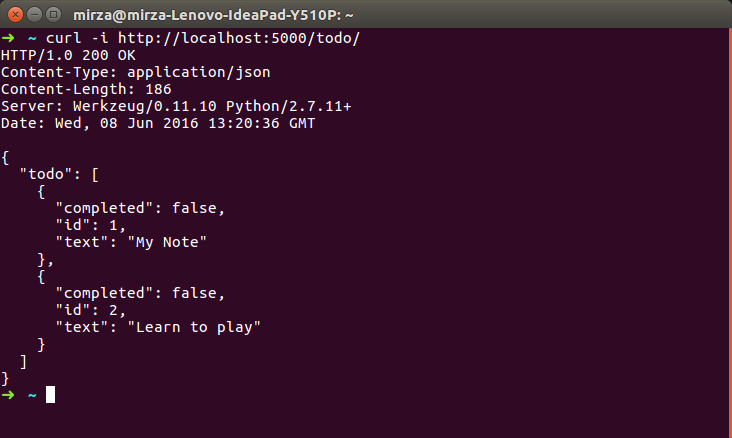
\includegraphics[scale=0.35]{GETAll.png}
  \caption{Example of GET to retrieve all todo tasks}\label{GETALL}
\end{figure}
But if I wish to only retrieve one specific ID, I can do this as well as shown in the picture below
\begin{figure}[H]
  \centering
  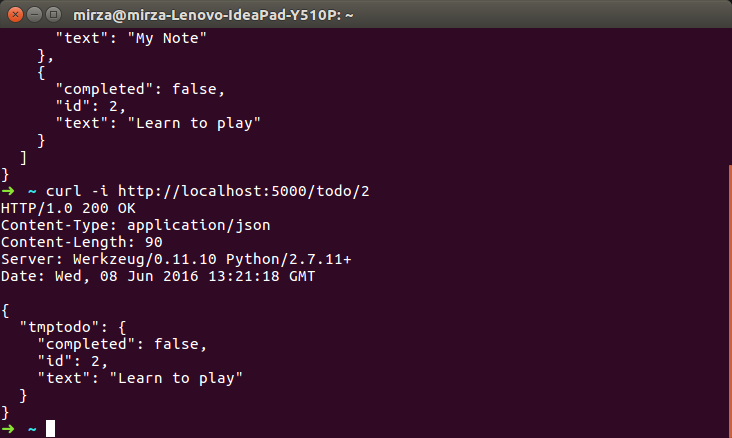
\includegraphics[scale=0.35]{GETID.png}
  \caption{Example of GET to retrieve ID 2}\label{GETID}
\end{figure}
I can also return errors if you try to call an ID that doesn't exist
\begin{figure}[H]
  \centering
  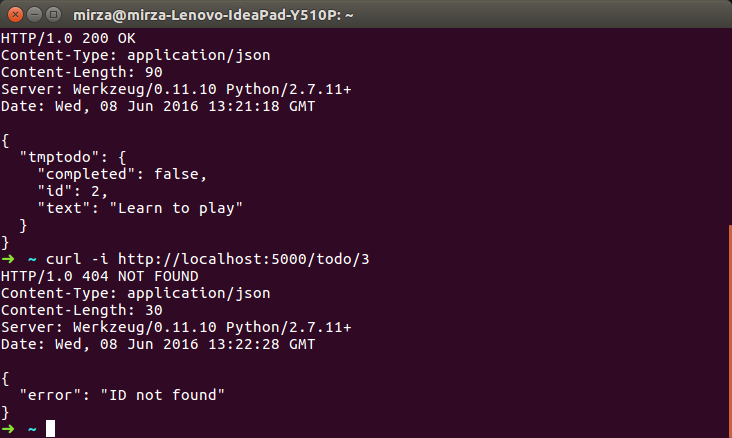
\includegraphics[scale=0.35]{GETIDnotfound.png}
  \caption{Example of GET to retrieve ID 3 but you get an error}\label{GETIDnotfound}
\end{figure}
I can as well POST a TODO if
\begin{figure}[H]
  \centering
  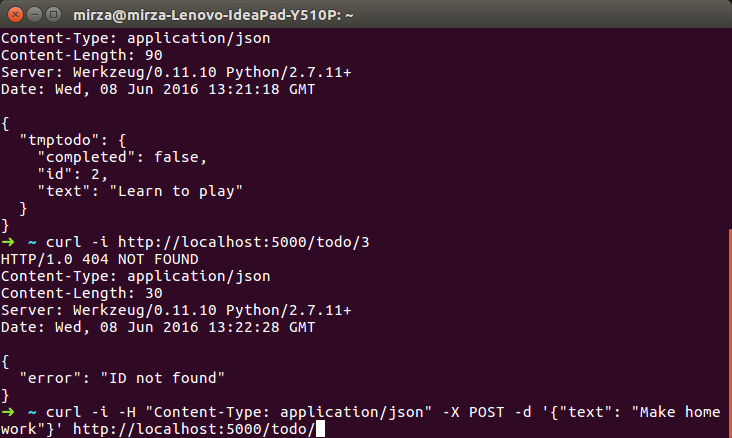
\includegraphics[scale=0.35]{POST.png}
  \caption{Example of POST}\label{POST}
\end{figure}
and if I call get of all the lists, you will see a new one, the one I created
\begin{figure}[H]
  \centering
  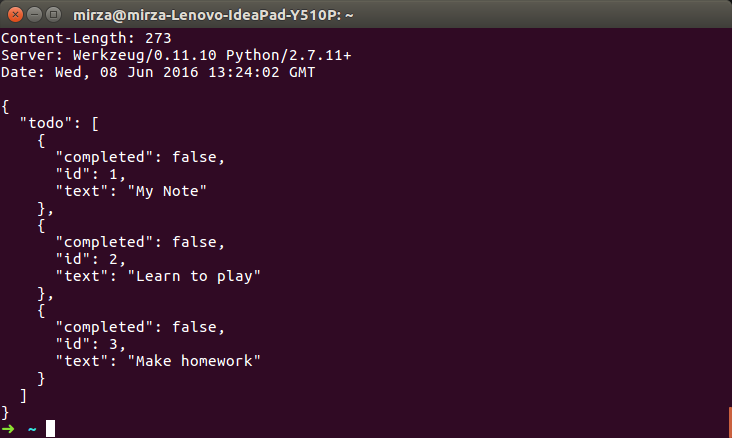
\includegraphics[scale=0.35]{GETafterPOST.png}
  \caption{Example of GET after using POST}\label{GETafterPOST}
\end{figure}
If I am done with a TODO I can update this TODO
\begin{figure}[H]
  \centering
  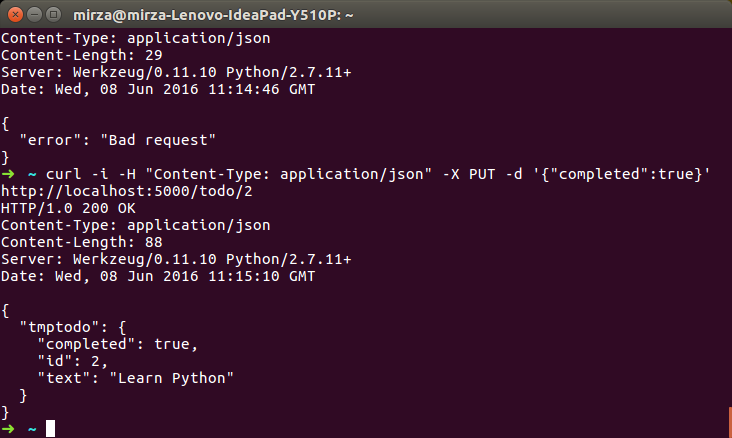
\includegraphics[scale=0.35]{PUTID2.png}
  \caption{Example of PUT on ID 2}\label{PUTID2}
\end{figure}
and now to see that it has been updated
\begin{figure}[H]
  \centering
  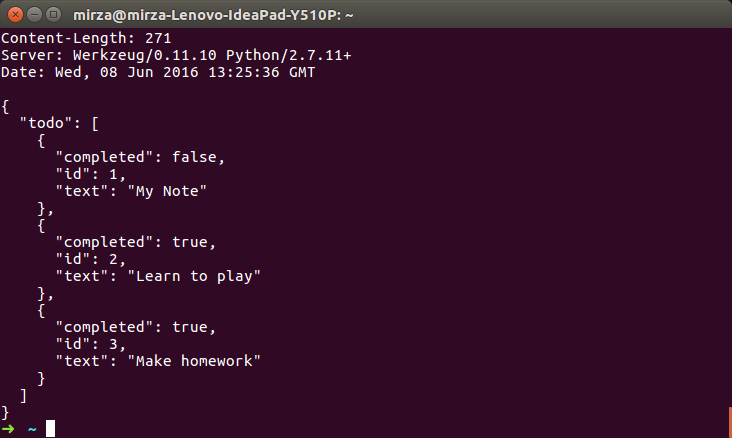
\includegraphics[scale=0.35]{GETafterPutID2.png}
  \caption{Example of PUT on ID 2 and now complete is True}\label{GETafterPutID2}
\end{figure}
and finally I can delete an ID
\begin{figure}[H]
  \centering
  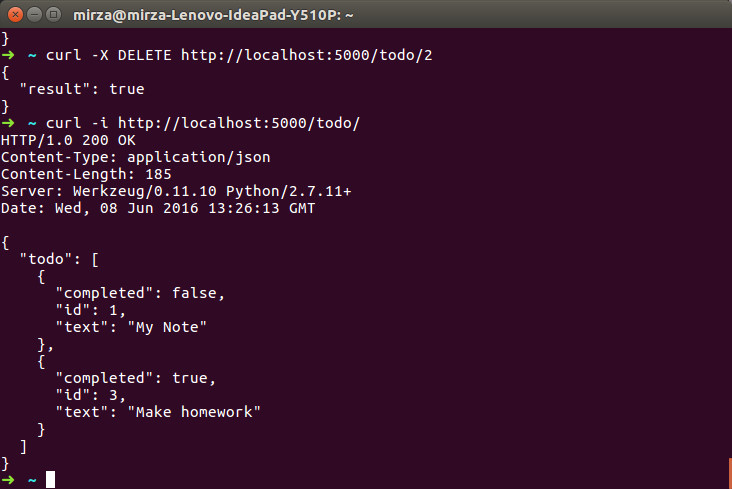
\includegraphics[scale=0.35]{DELETEID2.png}
  \caption{Example of DELETE}\label{DELETEID2}
\end{figure}

\section{Bottlenecks and limitation}
There are some limitation to this server. If I use the POST command I receive an error for some python that the dict are hashable. But I still manage to create a new TODO. 

The server is single threaded as mentioned earlier in this paper. But for this assignment I thought of it as okay, but if it was to be build in larger scale then the setup must be changed to be able to handle multi threading and multiple process.

Imagine that I have 3 TODO tasks with ID 1, 2 and 3. IF I delete ID 2, then I will have ID 1 and 3 left, the server will not update ID 3 to ID 2.

There is not implementation of a save command, to save your TODO tasks, so if the server restarts then everything will be lost

\section{Conclusion}
Overall the REST API is fine when to use as an API to handle CRUD operation on data and it is focused on accessing named resources through a single consistent interface.
REST is also good to use, because its simple and it permits many different data formats.

\newpage
\onecolumn
\appendix
%Appendix A
\section{Help to use web service}


\begin{table}[H]
  \centering
  \begin{tabular}{|c|c|c|c|}
    \hline
    % after \\: \hline or \cline{col1-col2} \cline{col3-col4} ...
    HTTP Method  & Action & Example \\ \hline
    GET &   Retrieve list of todo tasks & {\ssmall \texttt{curl -i http://localhost:5000/todo/} \par} \\ \hline
    GET &   Retrieve a todo task & {\ssmall \texttt{curl -i http://localhost:5000/todo/1} \par} \\ \hline
    POST &   Create a new todo task & {\tiny \texttt{curl -i -H "Content-Type: application/json" -X POST -d '\{"text":"some text"\}' http://localhost:5000/todo/} \par} \\ \hline
    PUT &   Update an existing todo task & {\tiny \texttt{curl -i -H "Content-Type: application/json" -X PUT -d '\{"completed":true\}' http://localhost:5000/todo/2} \par} \\ \hline
    DELETE &   Delete a todo task & {\ssmall \texttt{curl -X DELETE http://localhost:5000/todo/2} \par} \\
    \hline
  \end{tabular}
  \label{table:UsageOfass}
\end{table}

\normalsize

\end{document}
